\documentclass[xetex,mathserif,serif]{beamer}

\usepackage[log-declarations=false]{xparse}
\usepackage[quiet]{fontspec}
\usepackage{amsmath}
\usepackage{amsfonts}
\usepackage{enumerate}
\usepackage{polyglossia}
\usepackage{tikz}
\usetikzlibrary{arrows,shapes,trees}

% works for now
\setbeamertemplate{footline}{\insertframenumber/\inserttotalframenumber}

\setdefaultlanguage{spanish}

\begin{document}

  \begin{frame}
    \begin{center}
      \begin{block}{}
        Topología Algebraica
      \end{block}
      \begin{block}{}
        Ruben Astudillo
      \end{block}
    \end{center}

  \end{frame}

  \begin{frame}
    \frametitle{Motivación}

    \begin{block}{}
      Definir una invariante para espacios topológicos.
    \end{block}

    \pause

    \begin{block}{}
      Idea: Estudiar las curvas y las ``deformaciones'' admisibles entre
      ellas para un espacio dado.
    \end{block}
  \end{frame}

  \begin{frame}
    \frametitle{Curvas y homotopias}
    \begin{columns}

      \begin{column}{.5\textwidth}
        \begin{center}
          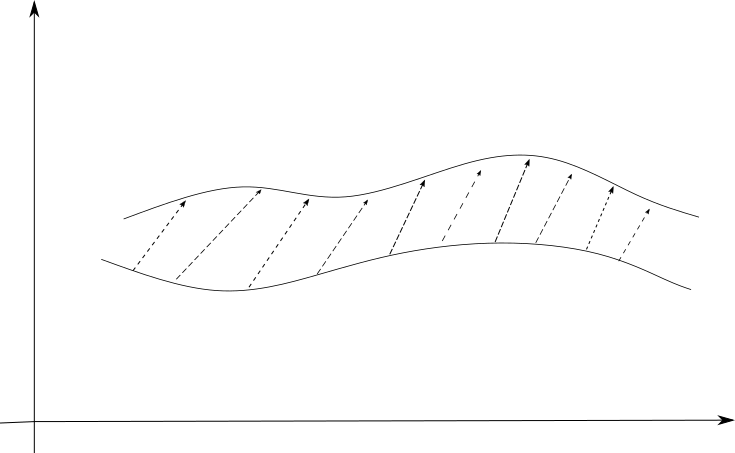
\includegraphics[scale=0.3]{../tesis/imagenes/homotopia.png}
        \end{center}
      \end{column}

      \pause

      \begin{column}{.5\textwidth}
        \begin{block}{Camino}
          Es una función continua \[ f : I \to X \] con \(X\) un espacio
          topológico
        \end{block}

        \pause

        \begin{block}{Homotopía entre \(f\) y \(g\)}
          Es una función continua \(H : I \times I \to X\) tal que
          \[ H(x,0) = f(x),\ H(x,1) = g(x) \]
          \[ f \sim g \]
        \end{block}
      \end{column}
    \end{columns}
  \end{frame}

  \begin{frame}
    \frametitle{Producto de caminos y homotopias}
    Si \(f (1) = g (0) \in X\) entonces el producto de caminos esta
    definido por
    \[ f * g (t) :=
      \begin{cases}
        f(2t) & t \in [0, \frac 1 2] \\
        g(2t - 1) & t \in [\frac 1 2 , 1 ]
      \end{cases}
    \]

    \begin{center}
      \begin{tikzpicture}[scale=0.8]
        \draw [blue, thick]  (0,0) to[bend right] (3,2) to[bend left] (4,3) ;
        \draw [red, thick] (4,3) to[bend right] (9,1) ;
      \end{tikzpicture}
    \end{center}

    \pause

    \begin{block}{}
      En general se consideran curvas con el mismo punto inicial y final
      (caminos cerrados).
    \end{block}
  \end{frame}

  \begin{frame}
    \frametitle{Producto de caminos y homotopias}
    Análogamente para homotopias \(F\) y \(G\) tal que \(H(1, t) =
    G(0,s) , \forall s, t \in I\), se define el producto de homotopias
    \[ F * G (x, t) :=
      \begin{cases}
        F(x, 2t) & t \in [0, \frac 1 2] \\
        G(x, 2t - 1) & t \in [\frac 1 2, 1]
      \end{cases}
    \]

    \pause

    \begin{center}
      \begin{tikzpicture}
        \draw[blue] (0,1) to[out=45, in=135] (3,1) ;
        \draw[blue] (0,1) to[out=25, in=155] (3,1) ;
        \draw[blue] (0,1) to[out=5, in=175] (3,1) ;
        \draw[blue] (0,1) to[out=-5, in=185] (3,1) ;
        \draw[blue] (0,1) to[out=-25, in=205] (3,1) ;
        \draw[blue] (0,1) to[out=-45, in=225] (3,1) ;

        \draw[red] (3,1) to[out=45, in=135] (7,2) ;
        \draw[red] (3,1) to[out=25, in=155] (7,2) ;
        \draw[red] (3,1) to[out=5, in=175] (7,2) ;
        \draw[red] (3,1) to[out=-5, in=185] (7,2) ;
        \draw[red] (3,1) to[out=-25, in=205] (7,2) ;
        \draw[red] (3,1) to[out=-45, in=225] (7,2) ;
      \end{tikzpicture}
    \end{center}
  \end{frame}

  \begin{frame}
    \frametitle{Grupo fundamental}
    \begin{block}{}
      Todo camino \(f : I \to X\) tiene un camino inverso \(\overline f (t)
      := f( 1 - t)\)
    \end{block}
    \begin{block}{}
      Se define el conjunto
      \[ \pi (X, x_0) := \{ [f] \mid f : I \to X ,\ f(0) = f(1) = x_0
        \} \]
      \[ [f] * [g] := [f * g]\]
      \[ g \in [f] \iff f \simeq g ,\ \text{ie existe una homotopía
          entre ellos}\]
    \end{block}

    \begin{block}{}
      La tupla \(
      \left(\pi(X, x_0), (*) \right) \) es llamado el grupo fundamental de \(X\).
    \end{block}
  \end{frame}

  \begin{frame}
    \frametitle{Importancia punto de origen}
    \begin{block}{}
      Esta invariante es útil en general solo para espacios arco-conexo
      pues queremos que la elección de punto \(x_0\) no afecte al grupo.
    \end{block}

    \pause

    \begin{block}{}
      El punto de origen igual se incluye por la caracterización de
      conmutatividad del grupo fundamental y tratamiento mas explicito con
      respecto a la teoría de cubrimientos.
    \end{block}
  \end{frame}
\end{document}
